\documentclass[border=20pt]{standalone}
\usepackage{tikz}
\begin{document}
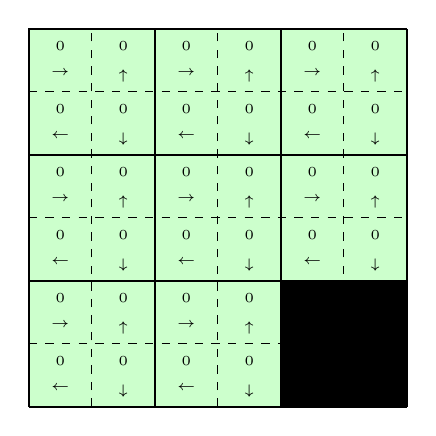
\begin{tikzpicture}[ scale=0.8]
	\path[draw, fill=green!20] (0, -6) -- (6, -6) -- (6, 0) -- (0, 0) -- cycle;
  	\path[draw, dashed] (0, -6) grid (6, 0);
	\path[draw, step=2, thick] (0, -6) grid (6, 0);
	
	def

	\foreach \x in {0.5, 1.5, 2.5, 3.5, 4.5, 5.5}
        \foreach \y in {-0.5, -1.5, -2.5, -3.5, -4.5, -5.5}
            \node[above] (x) at (\x, \y) {\tiny   0};
    
    
    
    \foreach \x in {0.5, 2.5, 4.5}
        \foreach \y in {-0.5, -2.5, -4.5}
            \node[below] (x) at (\x, \y) {\tiny $\rightarrow$};

    \foreach \x in {1.5, 3.5, 5.5}
        \foreach \y in {-0.5, -2.5, -4.5}
            \node[below] (x) at (\x, \y) {\tiny $\uparrow$};

    \foreach \x in {0.5, 2.5, 4.5}
        \foreach \y in {-1.5, -3.5, -5.5}
            \node[below] (x) at (\x, \y) {\tiny $\leftarrow$};

    \foreach \x in {1.5, 3.5, 5.5}
        \foreach \y in {-1.5, -3.5, -5.5}
            \node[below] (x) at (\x, \y) {\tiny $\downarrow$};
    
\path[draw, fill=black] (4, -6) -- (6, -6) -- (6, -4) -- (4, -4) -- cycle;

\end{tikzpicture}

\end{document}
